\documentclass[11pt, a4paper]{article}
\usepackage[utf8]{inputenc}
\usepackage[margin=.7in]{geometry}
\usepackage{listings}
\usepackage{setspace}
\usepackage{xcolor}
\usepackage{titlesec}
\usepackage{enumitem}
\usepackage{amssymb}
\usepackage{amsmath}
\usepackage{bm}
\usepackage{multicol}
\usepackage{graphicx}
\graphicspath{{./Figures/}}
\usepackage{color}
\usepackage{hyperref}
\hypersetup{
	colorlinks=true,
	linkcolor=blue,
	urlcolor=blue,
}
\titleformat*{\section}{\LARGE\bfseries\filcenter}
\titleformat*{\subsection}{\Large\bfseries}
\titleformat*{\subsubsection}{\large\bfseries}
\definecolor{codegreen}{rgb}{0,0.5,0}
\definecolor{codegray}{rgb}{0.5,0.5,0.5}
\definecolor{codered}{rgb}{0.78,0,0}
\definecolor{codepurple}{rgb}{0.58,0,0.68}
\definecolor{backcolour}{rgb}{0.95,0.95,0.92}
\lstdefinestyle{Pythonstyle}{
	language = Python,
    backgroundcolor=\color{backcolour},   
    commentstyle=\color{gray},
    keywordstyle=\color{codegreen},
    numberstyle=\tiny\color{codegray},
    stringstyle=\color{codered},
    basicstyle=\ttfamily\footnotesize,
    breakatwhitespace=false,         
    breaklines=true,                 
    captionpos=b,                    
    keepspaces=true,                 
    numbers=left,                    
    numbersep=5pt,                  
    showspaces=false,                
    showstringspaces=false,
    showtabs=false,                  
    tabsize=2,
    morekeywords = {as},
    keywordstyle = \color{codegreen}
}
\lstset{style=Pythonstyle}

\begin{document}
	\begin{titlepage}
		\begin{center} \Huge \textbf{Deep Learning in Python} \end{center}
		\tableofcontents
		\newpage
	\end{titlepage}
%%%% PAGE 1 %%%%

	\begin{spacing}{1.1}
	\section{Neural Networks and Deep Learning}
	\subsection{Logistic Regression as a Neural Network}
	\subsubsection{Introduction to Logistic Regression}
	\begin{minipage}[c]{10cm}
	A single \textbf{neural network} can be built off of an input (x), an activation layer known as a \textit{neuron}, and producing an output (y). A larger neural network is then formed by taking many of the single neurons and stacking them together. Each \textit{feature} ($x_1, x_2,..., x_n$) can be used as an input to the activation layers to produce our output y. For the below example, we say that the layer in the middle is \textit{densely connected} since every feature is in input.
	\end{minipage}
	\begin{minipage}[c]{4cm}
	\hspace*{6mm} 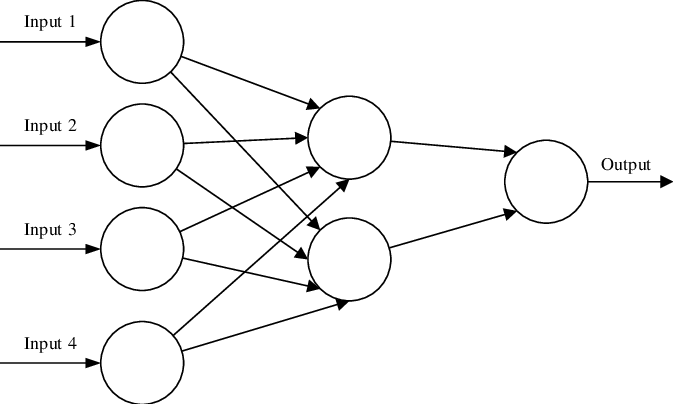
\includegraphics[scale=.25]{nn_intro} 
	\end{minipage} \vspace*{3mm} \\~\\
	To store an image, your computer stores three different matrices corresponding to the red, green, and blue channel (RGB values). So if your input image is 64x64 pixels, you will have three 64x64 matrices. To unroll these values into a \textbf{feature vector}, we will add values from all 3 vectors into a single x vector, where $n_x$ is the number of features in the vector (in this case, 12288). \vspace*{2mm} \\
	In \textbf{binary classification}, our goal is to learn a classifier that can input an image represented by feature vector \textit{x} and predict whether the corresponding label y is a 1 or 0 (1 for cat, 0 for non cat). \vspace*{2mm} \\
	Here is some common notation we will be using: \vspace*{1mm} \\
	\hspace*{3mm} - Single training example: (x,y) where $x \in \mathbb{R}^{n_x}$, y $\in \{0,1\} $ \vspace*{1mm} \\
	\hspace*{3mm} - M training examples: $\{(x^1, y^1), ..., (x^m, y^m)\}$  \vspace*{1mm} \\
	\hspace*{3mm} - Matrix X: $\begin{bmatrix} | & | & ... & | \\ x^1 & x^2 & ... & x^m \\ | & | & ... & | \end{bmatrix}$ where rows = $n_x$, columns = m. In Python, X.shape = ($n_x$, m). \vspace*{2mm} \\
	\hspace*{3mm} - Matrix Y: $\begin{bmatrix} y^1, y^2, ..., y^m \end{bmatrix}$ where Y.shape = (1, m) \\~\\
	Given x, we want an estimate known as $\hat{y}$ = P(y=1$|$x) given the following parameters: $x \in \mathbb{R}^{n_x}$, $w \in \mathbb{R}^{n_x}$, and $b \in \mathbb{R}$. We want out output to be $0 \leq \hat{y} \leq 1$, so we will use the \textbf{sigmoid function} to find our output, which will be: $$ \hat{y} = \sigma (z) \;\; \text{where}\;\; z = w^Tx + b \;\; \text{and}\;\; \sigma(z) = \frac{1}{1+e^{-z}}$$ If z is large, then $\sigma(z)$ will be very close to 1. But if z is a large negative number, then $\sigma(z)$ will be very close to 0. So given $\{(x^1, y^1),...,(x^m,y^m)\}$ we want $\hat{y}^i \approx y^i$
	\subsubsection{Logistic Regression Cost Function}
	We will associate $x^i$, $y^i$, and $z^i$ with the $i^{th}$ training example of our data. We will need to define a \textbf{loss function}, with respect to a single training example, to measure how good our output ($\hat{y}$) is when the true label is y. Since we are using gradient descent, we will define the following loss function: $$ \mathcal{L}(\hat{y},y) \; = \; -(y\,log(\hat{y}) \; + \; (1-y)\,log(1-\hat{y}))  $$ We want this loss function to be as small as possible. Lets look at the two cases: \vspace*{1mm} \\
	\hspace*{2mm} If y=1: $ \mathcal{L}(\hat{y},y) \, = \, -y\,log(\hat{y})$ and we want this to be as small as possible ($\hat{y}$ large). \\
	\hspace*{2mm} If y=0: $ \mathcal{L}(\hat{y},y) \, = \, -\,log(1-\hat{y})$ and we want this to be large ($\hat{y}$ small). \newpage
%%%% PAGE 2 %%%%

	\noindent To train the parameters \textit{w} and \textit{b}, we need to define a \textbf{cost function}, which measures how well your doing on an entire training set (cost of the parameters). We will define this as: \\ $$ J(w,b)\, = \, \frac{1}{m}\, \sum_{i=1}^{m}\, \mathcal{L}(\hat{y}^i,y^i) \; = \; -\frac{1}{m}\, \sum_{i=1}^{m}\, [(y^i\,log(\hat{y}^i) \; + \; (1-y^i)\,log(1-\hat{y}^i))] $$
	\subsubsection{Gradient Descent}
	\begin{minipage}[c]{10cm}
	We want to find the values of w and b that will \textit{minimize} the cost function J(w,b). Our cost function that we defined is convex (only one minimum). So we will initialize (w,b) to a random value, typically zero, and will take steps downhill in the steepest direction it can. Eventually it will converge to a minimum value and find our parameter values.
	\end{minipage}
	\begin{minipage}[c]{6cm}
	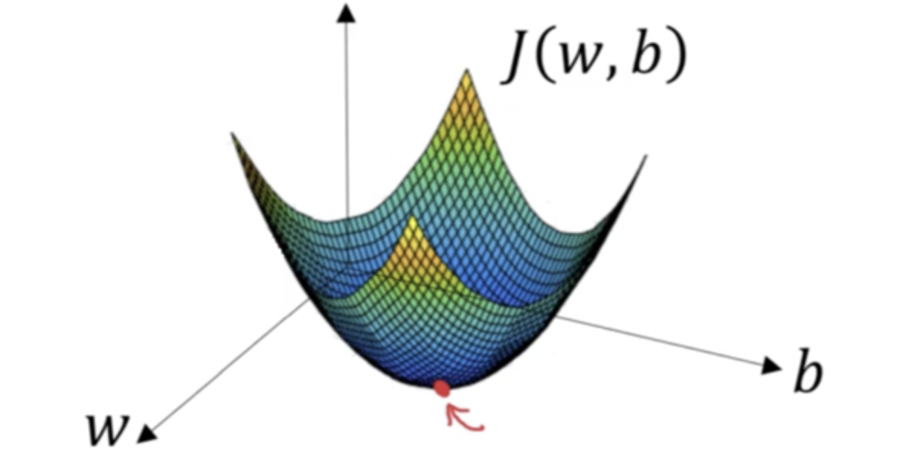
\includegraphics[scale=.4]{grad_desc}
	\end{minipage} \vspace*{4mm} \\~\\
	\textbf{Gradient descent} will repeatedly update the value of w and b with the formula: $$ w \, = \, w \, - \, \alpha \, \frac{ \partial J(w,b)}{\partial w} \; , \; b \, = \, b \, - \, \alpha \, \frac{\partial J(w,b)}{\partial b} $$ where $\alpha$ is our learning rate that we set multiplied by the partial derivative (since there are two variables) of the cost function with respect to the given parameter. \vspace*{2mm} \\
	We want to modify out \textit{w} and \textit{b} parameters in order to reduce the loss when performing gradient descent on our Logistic Regression. We can set up a computation graph to find the derivatives through \textbf{backpropagation}. We will do this for a \textit{single} training example, lets remind ourselves of our equations and the graph: \\
	\begin{minipage}[c]{8cm}
	$ z = w^Tx+ b$ \\
	$\hat{y} = a = \sigma(z)$ \\
	$\mathcal{L}(a,y) \; = \; -(y\,log(a) \; + \; (1-y)\,log(1-a))$ \\
	\end{minipage}
	\begin{minipage}[c]{6cm}
	\vspace*{2mm}
	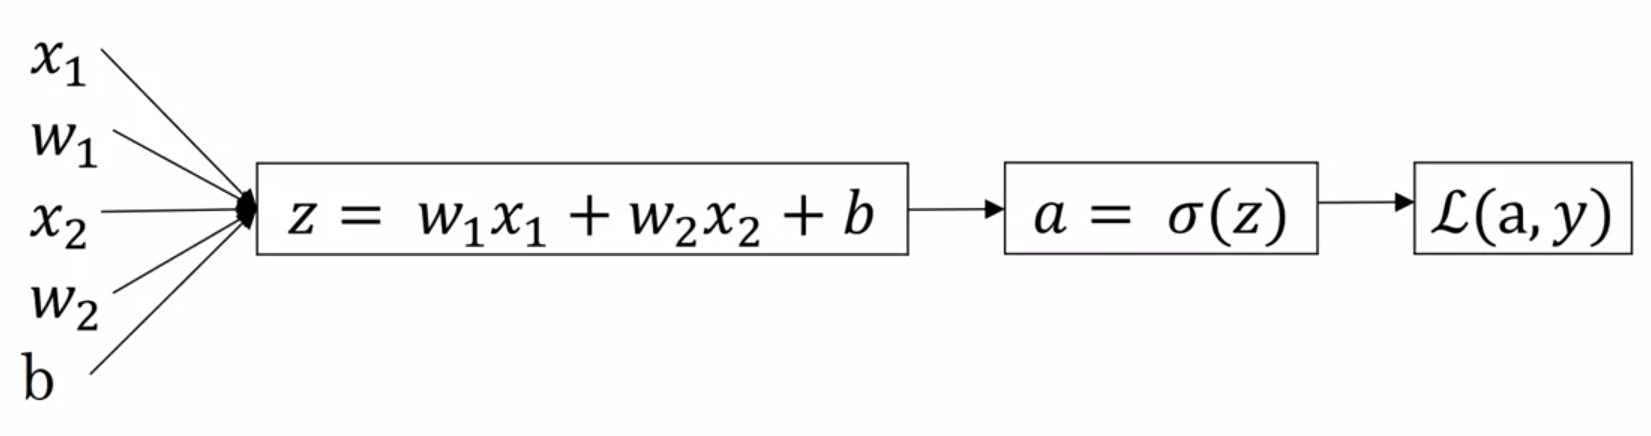
\includegraphics[scale=.2]{comp_graph}
	\end{minipage} \vspace*{1mm} \\~\\
	The first back step is to compute ``da'' = $\frac{\partial \mathcal{L}(a,y)}{\partial a}\; = \; \frac{-y}{a} - \frac{1-y}{1-a}$ \vspace*{2mm}\\
	Next we step back again and compute ``dz'' = $\frac{\partial \mathcal{L}(a,y)}{\partial z}\; = \; \frac{\partial \mathcal{L}}{\partial a}*\frac{\partial a}{\partial z}\; = \; a(1-a)*(\frac{-y}{a} + \frac{1-y}{1-a})\; = \; a-y$ \vspace*{2mm}\\
	The final step back is to find how much to change our $w_1$, $w_2$, and $b$ values. We can do this by: \vspace*{1mm} \\
	\hspace*{2mm} - Calculating: $\frac{\partial \mathcal{L}}{\partial w_1}\;$ = ``$dw_1$" = $x_1 * dz$, ``$dw_2$" = $x_2 * dz$, and ``$db$" = $dz$ \vspace*{1mm} \\
	\hspace*{2mm} - Then update our variables: $w_1 \; = \; w_1 - \alpha* dw_1$, $w_2 \; = \; w_2 - \alpha* dw_2$, and $b \; = \; b - \alpha* dz$ \\~\\
	Now we want to \textbf{perform gradient descent on m examples}. This will use the cost function (not the loss function like we did on a single example). We will write sudo-code for Python that implements this m example gradient descent: \\
	\begin{minipage}[c]{8cm}
	Initialize: J=0, $dw_1$=0, $dw_2$=0, db=0 \\
	for i=1 to m: \\
	\hspace*{2mm} $z^i = w^Tx^i+b$\\
	\hspace*{2mm} $z^i = \sigma(z^i)$\\
	\hspace*{2mm} $J+= -[(y^i\,log(a^i) \; + \; (1-y^i)\,log(1-a^i))]$\\
	\hspace*{2mm} $dz^i = a^i - y^i$\\
	\hspace*{2mm} $dw_1 += x_1^i*dz^i$\\
	\hspace*{2mm} $dw_2 += x_2^i*dz^i$\\
	\hspace*{2mm} $db += dz^i$
	\end{minipage}
	\begin{minipage}[c]{8cm}
	\vspace*{2mm}
	After the loop, we then take the average and update our varaibles: \vspace*{1mm} \\
	J /= m \\
	$dw_1$ /= m \\
	$dw_2$ /= m \\
	db /= m \vspace*{1mm} \\
	$w_1 \; = \; w_1 - \alpha* dw_1$ \\
	$w_2 \; = \; w_2 - \alpha* dw_2$\\
	 $b \; = \; b - \alpha* db$
	
	\end{minipage} \newpage
%%%% PAGE 3 %%%%

	\subsection{Vectorization in Python}
	
	
	
	
	
	
	
\end{spacing}
\end{document}